\documentclass{standalone}
\usepackage{tikz}
\usetikzlibrary{patterns, positioning}
\usepackage[sfdefault]{ClearSans} %% option 'sfdefault' activates Clear Sans as the default text font
\usepackage[T1]{fontenc}

\begin{document}
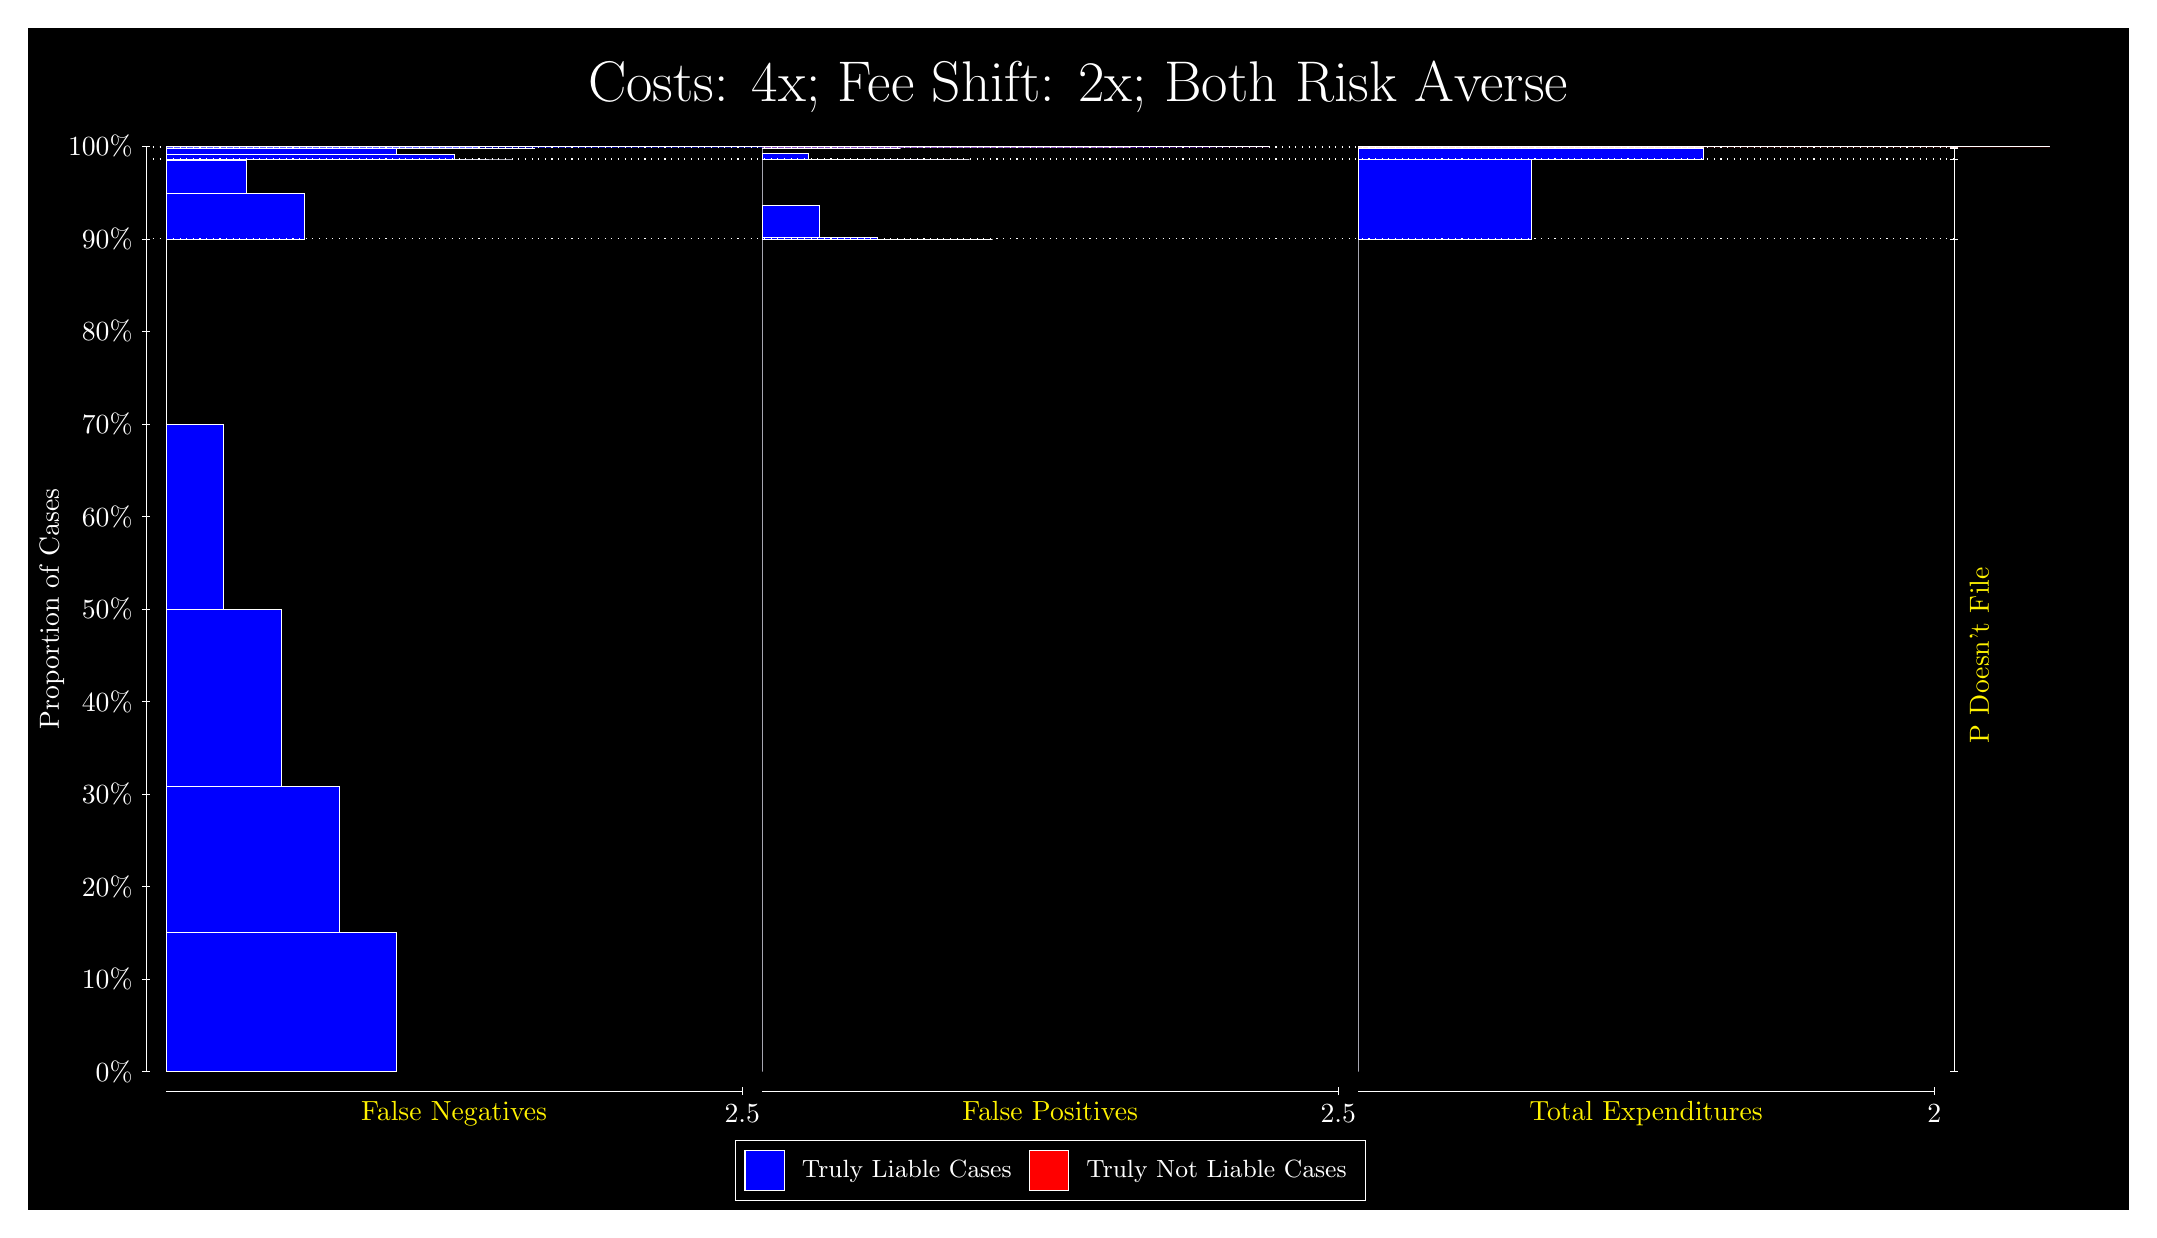
\begin{tikzpicture}
\draw[fill=black] (0,0) rectangle (26.667,15);
\draw[text=white] (0,13.5) rectangle (26.667,15) node[midway] {\huge Costs: 4x; Fee Shift: 2x; Both Risk Averse};
\draw[white, very thin] (1.5,1.75) -- (1.5,13.5);
\node[rotate=90, text=white, anchor=center] at (0.3, 7.625) {Proportion of Cases};
\draw[white, very thin] (1.45,1.75) -- (1.55,1.75);
\node[text=white, anchor=east] at (1.45, 1.75) {0\%};
\draw[white, very thin] (1.45,2.925) -- (1.55,2.925);
\node[text=white, anchor=east] at (1.45, 2.925) {10\%};
\draw[white, very thin] (1.45,4.1) -- (1.55,4.1);
\node[text=white, anchor=east] at (1.45, 4.1) {20\%};
\draw[white, very thin] (1.45,5.275) -- (1.55,5.275);
\node[text=white, anchor=east] at (1.45, 5.275) {30\%};
\draw[white, very thin] (1.45,6.45) -- (1.55,6.45);
\node[text=white, anchor=east] at (1.45, 6.45) {40\%};
\draw[white, very thin] (1.45,7.625) -- (1.55,7.625);
\node[text=white, anchor=east] at (1.45, 7.625) {50\%};
\draw[white, very thin] (1.45,8.8) -- (1.55,8.8);
\node[text=white, anchor=east] at (1.45, 8.8) {60\%};
\draw[white, very thin] (1.45,9.975) -- (1.55,9.975);
\node[text=white, anchor=east] at (1.45, 9.975) {70\%};
\draw[white, very thin] (1.45,11.15) -- (1.55,11.15);
\node[text=white, anchor=east] at (1.45, 11.15) {80\%};
\draw[white, very thin] (1.45,12.325) -- (1.55,12.325);
\node[text=white, anchor=east] at (1.45, 12.325) {90\%};
\draw[white, very thin] (1.45,13.5) -- (1.55,13.5);
\node[text=white, anchor=east] at (1.45, 13.5) {100\%};

\draw[white, very thin] (24.457,1.75) -- (24.457,13.5);
\draw[white, very thin] (24.407,1.75) -- (24.507,1.75);
\node[anchor=west] at (24.407, 1.75) {};
\draw[white, very thin] (24.407,12.325) -- (24.507,12.325);
\node[anchor=west] at (24.407, 12.325) {};
\draw[white, very thin] (24.407,13.339) -- (24.507,13.339);
\node[anchor=west] at (24.407, 13.339) {};
\draw[white, very thin] (24.407,13.48) -- (24.507,13.48);
\node[anchor=west] at (24.407, 13.48) {};
\draw[white, very thin] (24.407,13.491) -- (24.507,13.491);
\node[anchor=west] at (24.407, 13.491) {};
\draw[white, very thin] (24.407,13.497) -- (24.507,13.497);
\node[anchor=west] at (24.407, 13.497) {};
\draw[white, very thin] (24.407,13.5) -- (24.507,13.5);
\node[anchor=west] at (24.407, 13.5) {};

\draw[white, very thin, fill=blue] (1.75,1.75) rectangle (4.6775,3.5134);
\draw[white, very thin, fill=blue] (1.75,3.5134) rectangle (3.9457,5.3692);
\draw[white, very thin, fill=blue] (1.75,5.3692) rectangle (3.2138,7.6261);
\draw[white, very thin, fill=blue] (1.75,7.6261) rectangle (2.4819,9.9753);
\draw[white, very thin, fill=red] (1.75,9.9753) rectangle (1.75,9.9753);
\draw[white, very thin, fill=blue] (1.75,9.9753) rectangle (1.75,12.325);
\draw[white, very thin, fill=blue] (1.75,12.325) rectangle (3.5065,12.91);
\draw[white, very thin, fill=blue] (1.75,12.91) rectangle (2.7746,13.324);
\draw[white, very thin, fill=blue] (1.75,13.324) rectangle (2.0428,13.339);
\draw[white, very thin, fill=red] (1.75,13.339) rectangle (1.75,13.339);
\draw[white, very thin, fill=blue] (1.75,13.339) rectangle (1.75,13.339);
\draw[white, very thin, fill=blue] (1.75,13.339) rectangle (6.1413,13.339);
\draw[white, very thin, fill=blue] (1.75,13.339) rectangle (5.8486,13.339);
\draw[white, very thin, fill=blue] (1.75,13.339) rectangle (5.5558,13.339);
\draw[white, very thin, fill=blue] (1.75,13.339) rectangle (5.4094,13.402);
\draw[white, very thin, fill=blue] (1.75,13.402) rectangle (5.1167,13.403);
\draw[white, very thin, fill=blue] (1.75,13.403) rectangle (4.8239,13.403);
\draw[white, very thin, fill=blue] (1.75,13.403) rectangle (4.6775,13.479);
\draw[white, very thin, fill=blue] (1.75,13.479) rectangle (4.3848,13.479);
\draw[white, very thin, fill=blue] (1.75,13.479) rectangle (4.092,13.479);
\draw[white, very thin, fill=blue] (1.75,13.479) rectangle (3.9457,13.48);
\draw[white, very thin, fill=blue] (1.75,13.48) rectangle (3.6529,13.48);
\draw[white, very thin, fill=blue] (1.75,13.48) rectangle (3.3602,13.48);
\draw[white, very thin, fill=blue] (1.75,13.48) rectangle (3.2138,13.48);
\draw[white, very thin, fill=blue] (1.75,13.48) rectangle (2.921,13.48);
\draw[white, very thin, fill=blue] (1.75,13.48) rectangle (2.6283,13.48);
\draw[white, very thin, fill=red] (1.75,13.48) rectangle (1.75,13.48);
\draw[white, very thin, fill=blue] (1.75,13.48) rectangle (6.4341,13.48);
\draw[white, very thin, fill=blue] (1.75,13.48) rectangle (5.7022,13.489);
\draw[white, very thin, fill=blue] (1.75,13.489) rectangle (4.9703,13.491);
\draw[white, very thin, fill=blue] (1.75,13.491) rectangle (4.2384,13.491);
\draw[white, very thin, fill=blue] (1.75,13.491) rectangle (3.5065,13.491);
\draw[white, very thin, fill=red] (1.75,13.491) rectangle (1.75,13.491);
\draw[white, very thin, fill=blue] (1.75,13.491) rectangle (3.5065,13.491);
\draw[white, very thin, fill=blue] (1.75,13.491) rectangle (2.7746,13.497);
\draw[white, very thin, fill=blue] (1.75,13.497) rectangle (2.0428,13.497);
\draw[white, very thin, fill=red] (1.75,13.497) rectangle (1.75,13.497);
\draw[white, very thin, fill=blue] (1.75,13.497) rectangle (1.75,13.497);
\draw[white, very thin, fill=blue] (1.75,13.497) rectangle (15.217,13.497);
\draw[white, very thin, fill=blue] (1.75,13.497) rectangle (14.485,13.497);
\draw[white, very thin, fill=blue] (1.75,13.497) rectangle (13.753,13.497);
\draw[white, very thin, fill=blue] (1.75,13.497) rectangle (13.021,13.497);
\draw[white, very thin, fill=blue] (1.75,13.497) rectangle (12.289,13.497);
\draw[white, very thin, fill=blue] (1.75,13.497) rectangle (7.4587,13.497);
\draw[white, very thin, fill=blue] (1.75,13.497) rectangle (6.7268,13.497);
\draw[white, very thin, fill=blue] (1.75,13.497) rectangle (5.9949,13.498);
\draw[white, very thin, fill=blue] (1.75,13.498) rectangle (5.2631,13.499);
\draw[white, very thin, fill=blue] (1.75,13.499) rectangle (4.5312,13.5);
\draw[white, very thin, fill=blue] (1.75,13.5) rectangle (3.7993,13.5);
\draw[white, very thin, fill=blue] (1.75,13.5) rectangle (3.0674,13.5);
\draw[white, very thin, fill=blue] (1.75,13.5) rectangle (2.3355,13.5);
\draw[white, very thin, fill=red] (1.75,13.5) rectangle (1.75,13.5);
\draw[white, very thin, fill=red] (9.3189,1.75) rectangle (9.3189,1.75);
\draw[white, very thin, fill=blue] (9.3189,1.75) rectangle (9.3189,12.325);
\draw[white, very thin, fill=red] (9.3189,12.325) rectangle (12.246,12.325);
\draw[white, very thin, fill=blue] (9.3189,12.325) rectangle (12.246,12.325);
\draw[white, very thin, fill=blue] (9.3189,12.325) rectangle (11.515,12.325);
\draw[white, very thin, fill=blue] (9.3189,12.325) rectangle (10.783,12.34);
\draw[white, very thin, fill=blue] (9.3189,12.34) rectangle (10.051,12.754);
\draw[white, very thin, fill=blue] (9.3189,12.754) rectangle (9.3189,13.339);
\draw[white, very thin, fill=red] (9.3189,13.339) rectangle (11.954,13.339);
\draw[white, very thin, fill=blue] (9.3189,13.339) rectangle (11.954,13.339);
\draw[white, very thin, fill=red] (9.3189,13.339) rectangle (11.661,13.339);
\draw[white, very thin, fill=blue] (9.3189,13.339) rectangle (11.661,13.339);
\draw[white, very thin, fill=red] (9.3189,13.339) rectangle (11.368,13.339);
\draw[white, very thin, fill=blue] (9.3189,13.339) rectangle (11.368,13.339);
\draw[white, very thin, fill=blue] (9.3189,13.339) rectangle (11.222,13.339);
\draw[white, very thin, fill=blue] (9.3189,13.339) rectangle (10.929,13.339);
\draw[white, very thin, fill=blue] (9.3189,13.339) rectangle (10.636,13.34);
\draw[white, very thin, fill=blue] (9.3189,13.34) rectangle (10.49,13.34);
\draw[white, very thin, fill=blue] (9.3189,13.34) rectangle (10.197,13.34);
\draw[white, very thin, fill=blue] (9.3189,13.34) rectangle (9.9044,13.415);
\draw[white, very thin, fill=blue] (9.3189,13.415) rectangle (9.758,13.416);
\draw[white, very thin, fill=blue] (9.3189,13.416) rectangle (9.4652,13.417);
\draw[white, very thin, fill=blue] (9.3189,13.417) rectangle (9.3189,13.48);
\draw[white, very thin, fill=red] (9.3189,13.48) rectangle (11.075,13.48);
\draw[white, very thin, fill=blue] (9.3189,13.48) rectangle (11.075,13.48);
\draw[white, very thin, fill=blue] (9.3189,13.48) rectangle (10.344,13.48);
\draw[white, very thin, fill=blue] (9.3189,13.48) rectangle (9.6116,13.482);
\draw[white, very thin, fill=blue] (9.3189,13.482) rectangle (9.3189,13.491);
\draw[white, very thin, fill=red] (9.3189,13.491) rectangle (14.003,13.491);
\draw[white, very thin, fill=blue] (9.3189,13.491) rectangle (14.003,13.491);
\draw[white, very thin, fill=blue] (9.3189,13.491) rectangle (13.271,13.491);
\draw[white, very thin, fill=blue] (9.3189,13.491) rectangle (12.539,13.492);
\draw[white, very thin, fill=blue] (9.3189,13.492) rectangle (11.807,13.497);
\draw[white, very thin, fill=blue] (9.3189,13.497) rectangle (11.075,13.497);
\draw[white, very thin, fill=red] (9.3189,13.497) rectangle (15.759,13.497);
\draw[white, very thin, fill=blue] (9.3189,13.497) rectangle (15.759,13.497);
\draw[white, very thin, fill=blue] (9.3189,13.497) rectangle (15.028,13.497);
\draw[white, very thin, fill=red] (9.3189,13.497) rectangle (15.028,13.497);
\draw[white, very thin, fill=blue] (9.3189,13.497) rectangle (15.028,13.497);
\draw[white, very thin, fill=blue] (9.3189,13.497) rectangle (14.296,13.497);
\draw[white, very thin, fill=red] (9.3189,13.497) rectangle (14.296,13.497);
\draw[white, very thin, fill=blue] (9.3189,13.497) rectangle (14.296,13.497);
\draw[white, very thin, fill=blue] (9.3189,13.497) rectangle (13.564,13.498);
\draw[white, very thin, fill=red] (9.3189,13.498) rectangle (13.564,13.498);
\draw[white, very thin, fill=blue] (9.3189,13.498) rectangle (13.564,13.498);
\draw[white, very thin, fill=blue] (9.3189,13.498) rectangle (12.832,13.498);
\draw[white, very thin, fill=blue] (9.3189,13.498) rectangle (12.832,13.499);
\draw[white, very thin, fill=blue] (9.3189,13.499) rectangle (12.1,13.5);
\draw[white, very thin, fill=blue] (9.3189,13.5) rectangle (11.368,13.5);
\draw[white, very thin, fill=blue] (9.3189,13.5) rectangle (10.636,13.5);
\draw[white, very thin, fill=red] (9.3189,13.5) rectangle (9.3189,13.5);
\draw[white, very thin, fill=blue] (9.3189,13.5) rectangle (9.3189,13.5);
\draw[white, very thin, fill=red] (16.888,1.75) rectangle (16.888,1.75);
\draw[white, very thin, fill=blue] (16.888,1.75) rectangle (16.888,12.325);
\draw[white, very thin, fill=red] (16.888,12.325) rectangle (19.083,12.325);
\draw[white, very thin, fill=blue] (16.888,12.325) rectangle (19.083,13.339);
\draw[white, very thin, fill=red] (16.888,13.339) rectangle (21.279,13.339);
\draw[white, very thin, fill=blue] (16.888,13.339) rectangle (21.279,13.48);
\draw[white, very thin, fill=red] (16.888,13.48) rectangle (21.279,13.48);
\draw[white, very thin, fill=blue] (16.888,13.48) rectangle (21.279,13.491);
\draw[white, very thin, fill=red] (16.888,13.491) rectangle (21.279,13.491);
\draw[white, very thin, fill=blue] (16.888,13.491) rectangle (21.279,13.497);
\draw[white, very thin, fill=red] (16.888,13.497) rectangle (25.67,13.497);
\draw[white, very thin, fill=blue] (16.888,13.497) rectangle (25.67,13.498);
\draw[white, very thin, fill=red] (16.888,13.498) rectangle (25.67,13.498);
\draw[white, very thin, fill=blue] (16.888,13.498) rectangle (25.67,13.5);
\draw[white, very thin, fill=red] (16.888,13.5) rectangle (25.67,13.5);
\draw[white, very thin, fill=blue] (16.888,13.5) rectangle (25.67,13.5);
\draw[white, dotted] (1.5,12.325) -- (24.457,12.325);
\draw[white, dotted] (1.5,13.339) -- (24.457,13.339);
\draw[white, dotted] (1.5,13.48) -- (24.457,13.48);
\draw[white, dotted] (1.5,13.491) -- (24.457,13.491);
\draw[white, dotted] (1.5,13.497) -- (24.457,13.497);
\draw[white, very thin] (1.75,1.5) -- (9.0689,1.5);
\node[text=yellow, anchor=north] at (5.4094, 1.5) {False Negatives};
\draw[white, very thin] (9.0689,1.45) -- (9.0689,1.55);
\node[text=white, anchor=north] at (9.0689, 1.45) {2.5};

\draw[white, very thin] (9.3189,1.5) -- (16.638,1.5);
\node[text=yellow, anchor=north] at (12.978, 1.5) {False Positives};
\draw[white, very thin] (16.638,1.45) -- (16.638,1.55);
\node[text=white, anchor=north] at (16.638, 1.45) {2.5};

\draw[white, very thin] (16.888,1.5) -- (24.207,1.5);
\node[text=yellow, anchor=north] at (20.547, 1.5) {Total Expenditures};
\draw[white, very thin] (24.207,1.45) -- (24.207,1.55);
\node[text=white, anchor=north] at (24.207, 1.45) {2};

\node[text=yellow, centered, rotate=90] at (24.777, 7.0376) {P Doesn't File};






\draw (12.978300999999998,1.5) node[draw=none] (baseCoordinate) {};
\begin{scope}[align=center]
        \matrix[scale=0.5, draw=white, below=0.5cm of baseCoordinate, nodes={draw}, column sep=0.1cm]{
            \node[rectangle, draw, minimum width=0.5cm, minimum height=0.5cm, fill=blue] {}; &
            \node[draw=none, font=\small, text=white] (B) {Truly Liable Cases}; &
            \node[rectangle, draw, minimum width=0.5cm, minimum height=0.5cm, fill=red] {}; &
            \node[draw=none, font=\small, text=white] (B) {Truly Not Liable Cases}; \\
            };
\end{scope}

\end{tikzpicture}
\end{document}